\documentclass[12pt]{article}

\usepackage{fullpage}
\usepackage{graphicx}

\pagenumbering{gobble}

\begin{document}

\begin{center}
{\large\sf\textbf{FMiTF: Track l: Combining Formal, Static, and
  Dynamic Analysis to Verify and Validate Real-World Embedded Systems: Facilities, Equipment \& other Resources}}
\end{center}

\section*{Computing equipment}

The primary equipment used in this project will be standard workstations and commodity computing equipment; e.g., for development and analysis work, high-end workstations or even laptops will suffice, in line with current development practices in industry and research. Northern Arizona University has the usual high-end network and computing infrastructure for standard computing uses.  Should the need for more ambitious computing requirements arise, Northern Arizona University provides access to powerful additional computing infrastructure, also available to this project.  We also expect analysis to primarily be performed outside of the actual embedded environment.  If any more unusual computing needs arise, NAU has several ways to meet these needs, discussed below.

AEGIS is a private cloud computing facility being developed collaboratively by the University of Arizona (UA), Northern Arizona University, and Arizona State University (ASU) with the support of the Arizona Board of Regents. AEGIS is based on the NSF-supported iPlant (now CyVerse) cyberinfrastructure (http://www.iplantcollaborative.org) ) and provides cloud-based services to researchers and educators in the environmental and ecological sciences. It uses the NSF-supported iRODS (www.irods.org) distributed storage service and the OpenStack open-source cloud operating system, enabling researchers to develop custom images that support scientific workflows and deploy them as virtual machines in to the AEGIS cloud for execution. NAU’s AEGIS hardware platform is networked with servers at UA and ASU and consists of a storage server with 2 X Intel Xeon E5-2620 2.00 GHz 8-core processors, 64 GB of DDR3 ECC memory, and 96 TB of disk storage in a RAID-6 configuration.

NAU’s Monsoon high-performance computing facility is a capacity-type, Linux-based computer cluster with 2860 Intel Xeon cores, 24TB of memory, and 16 NVIDIA GPUs: K80, and P100. It has been designed to be flexible and handle a diverse set of research requirements. 103 individual systems are interconnected via FDR Infiniband at a rate of 56Gbps and $<.07$us latency. Cluster nodes have access to 1.3PB of shared storage of type scratch (lustre), and long-term project space (ZFS). Monsoon has a measured peak performance of 107 teraflops. It is housed in the NAU ITS Server Co-Location Room, which contains the necessary power and other facilities requirements such as a non-water fire suppression system.


\section*{DISCOVER/Robotics}

For the DISCOVER wireless sensor networks and robotics case studies, the DISCOVER project and the Intelligent Control Systems Lab at NAU will provide all the necessary equipment and infrastructure for the studies, with no needs specific to this project.
That includes over 180 wireless sensor nodes with edge computing capability (Figure~\ref{fig:discover}, left), 15 rovers (Figure~\ref{fig:discover}, center), 10 drones (Figure~\ref{fig:discover}, right), embedded computers, computing servers, and all required software, which are distributed and coordinated over four sites in Arizona, New Mexico, and South Carolina.
The sites are also equipped with last-mile connectivity, including software defined radios (SDR). % operating over the Citizen Broadcast Radio Services (CBRS) spectrum ($3.5-3.7$ (GHz)).
These equipment and resources will support the proposed research, validation, and education activities.

\begin{figure}[!ht]
  % \centering
  % \vspace{-8pt}
  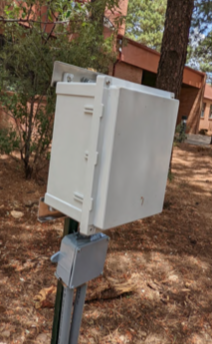
\includegraphics[height=3.5cm]{figs/discover-node.png}
  \hfill
  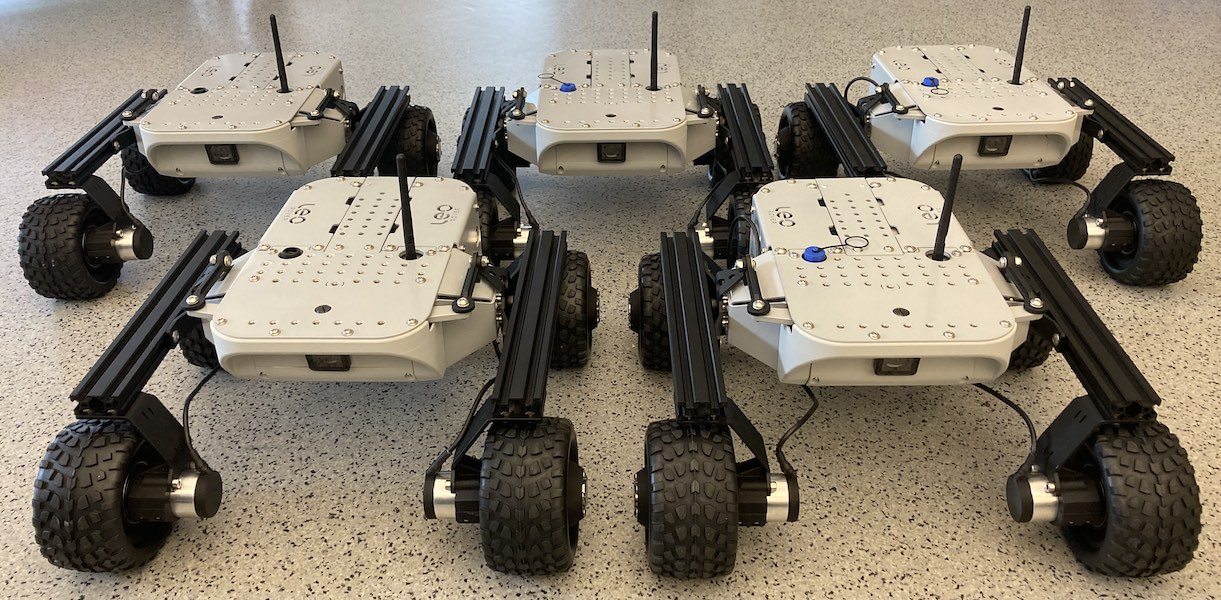
\includegraphics[height=3.5cm]{figs/discover-rovers.jpg}
  \hfill
  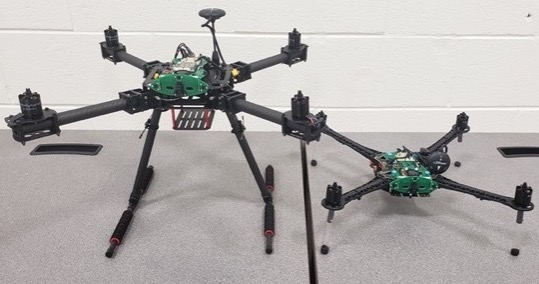
\includegraphics[height=3.5cm]{figs/discover-drone.jpg}
  \caption{DISCOVER infrastructure: a wireless sensor node (left), some rovers (center), and some drones (right).}
  \label{fig:discover}
\end{figure}

\subsection*{Programs at NAU for Recruiting Research Students}

NAU has been providing many opportunities and programs supporting students in higher education and in research, especially underrepresented minorities.
Described below are some relevant programs.
\begin{itemize}
\item The \textsl{Interns-to-Scholars} (I2S) program seeks to encourage undergraduate students early in their academic careers to participate in %faculty
  research %, scholarly, or creative projects
  by working as paid interns, for up to 20 hours/week during a semester.
  Internships across all academic disciplines offer opportunities for students to engage in ``learning by doing'' outside of regular coursework.
  Beyond the internship, I2S students have access to professional development workshops that guide them through processes such as developing and delivering technical research presentations, writing research manuscripts, and pursuing research funding.
  % Co-PI~Nghiem has mentored several I2S students at NAU.

\item The \textsl{NSF Southern Nevada Northern Arizona Louis Stokes Alliance for Minority Participation} (LSAMP) program supports underrepresented minority students pursuing degrees in STEM through a comprehensive approach to student development, community building and career readiness.  It helps faculty members recruit minority research students and provides funding for these students to participate in research.
  %Co-PI~Nghiem has mentored one LSAMP students at NAU.

\item The \textsl{National Graduate Education for Minorities (GEM) Consortium} recruits and provides fellowships for underrepresented students pursuing graduate degrees.  NAU is a university member of GEM and Co-PI~Nghiem is a representative of NAU at GEM.
\end{itemize}

\end{document}
